\subsection[Neumann Zyklus]{Von Neumann Zyklus}
\label{subsec:Neumann-Zyklus}

Der Von Neumann Zyklus der UMach ist auf 4 Schritte verkürzt. Dies ist möglich,
da die Instruktionsbreite immer aus 4 Wörtern besteht, und somit der 
\glqq\textsc{Fetch}\grqq\ von 
Befehl und zugehörigen Operanden in einem gemeinsamen Schritt durchgeführt
werden kann. Somit besteht der Zyklus aus einem beginnenden \textsc{Fetch}. Bei
diesem wird der an der im Programmcounter \texttt{PC} liegende Adresse
gespeicherte Befehl in das Instruktionsregister \texttt{IR} geladen. Danach
wird der im ersten Byte liegende Befehl mit Hilfe des Befehlsdecoders decodiert
und an der \textsc{ALU} entsprechend eingestellt. 

In einem dritten Schritt \textsc{Execute} wird die Instruktion ausgeführt. Der
theoretisch 4. Schritt, das Inkrementieren des Programmcounters \texttt{PC},
wird parallel zu den \textsc{Fetch} und \textsc{Decode} Vorgängen ausgeführt.
Diese Tatsache ist bei Instruktionen, welche den Inhalt des \texttt{PC}
manipulieren, zu berücksichtigen. Siehe auch Abbildung \ref{fig:Neumann-Zyklus}
auf Seite \pageref{fig:Neumann-Zyklus}.

Auflistung der Schritte:

\begin{enumerate}
 \item \textsc{Fetch} --
       Holen der Instruktion aus dem Speicher an der im \texttt{PC} vorliegenden Adresse.
 \item \textsc{Decode} --
       Decodieren des Befehles und Einstellen der \textsc{ALU}.
 \item \textsc{Execute} --
       Auführen des Befehles in der \textsc{ALU}.
 \item \textsc{Update} \texttt{PC} --
       Inkrementieren des \texttt{PC}. Findet parallel zu \textsc{Fetch} und
       \textsc{Decode} statt.
\end{enumerate}

\begin{figure}[h!tp]
 \centering
 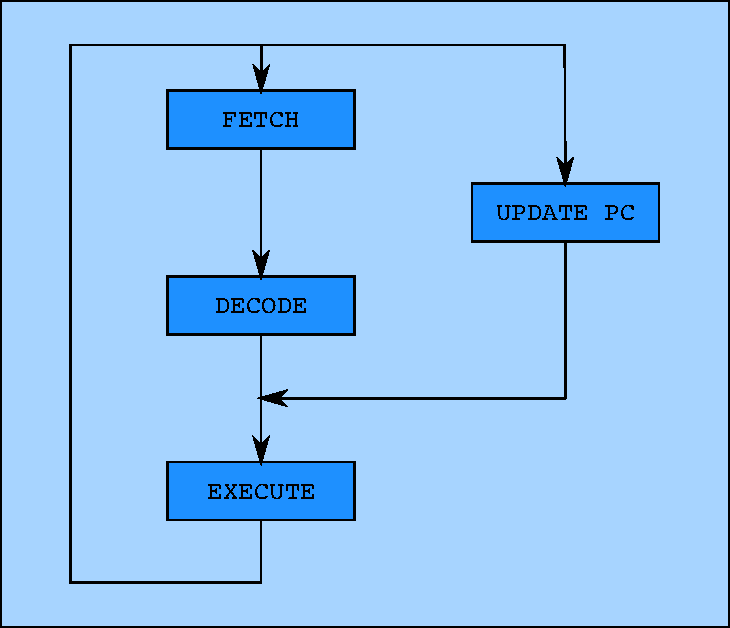
\includegraphics{./img/zyklus.pdf}
 \caption{Von Neumann Zyklus }
 \label{fig:Neumann-Zyklus}
\end{figure}

